\section{Tổng kết}
\subsection{Kết quả đạt được}
\subsubsection{Đối với tìm hiểu và phân tích nghiệp vụ}
Căn cứ vào mục tiêu, nhiệm vụ đã đề ra, nhóm tác giả đã phân tích hoàn chỉnh nghiệp vụ của hệ
thống:
\begin{itemize}
    \item Tiến hành phân tích tất cả các yêu cầu cần có của hệ thống, kết hợp so sánh với các hệ thống tương
    tự đã có trên thị trường và rút ra được các ưu, nhược điểm của các hệ thống đó.
    \item Bổ sung các tính năng mới mà các ứng dụng tương tự hiện nay chưa có hoặc chưa tích hợp vào hệ
    thống của họ cũng như cải thiện các tính năng mà các hệ thống đó làm chưa tốt.
    \item Xác định được các stakeholder liên quan đến hệ thống, đồng thời phân tích được nhu cầu và ảnh hưởng của họ đối với hệ thống.
    \item Xác định đầy đủ vai trò của từng loại người dùng trong hệ thống và phân tích chi tiết các user
    story của họ.
    \item Phân tích được các yêu cầu chức năng và phi chức năng mà hệ thống cần phải có.
\end{itemize}
\subsubsection{Đối với cơ sở lý thuyết và công nghệ}
Dựa vào các quy tắc nghiệp vụ và các yêu cầu phân tích được của hệ thống, nhóm đã tiến hành tìm
hiểu tất cả các khái niệm và các công nghệ để sử dụng trong hệ thống:
\begin{itemize}
    \item Tìm hiểu về các khái niệm quan trọng và cách thức hoạt động của chatbot AI.
    \item Tìm hiểu về các mô hình ngôn ngữ lớn phục vụ cho chatbot trả lời tự động như GPT, DialoGPT,
    BERT, T5, BlenderBot, Llama.
    \item Chọn được các ngôn ngữ lập trình, framework và các công nghệ phù hợp để xây dựng hệ thống bao gồm các công nghệ cho Frontend, Backend và AI.
    \item Lựa chọn công nghệ và thực hiện triển khai hệ thống với các tính năng hiện có.
\end{itemize}
\subsubsection{Đối với phân tích và thiết kế hệ thống}
Dựa vào các quy tắc nghiệp vụ, các yêu cầu phân tích được của hệ thống, nhóm đã thực hiện phân tích hệ thống theo các lược đồ, đồng thời hoàn thành giai đoạn thiết kế hệ thống:
\begin{itemize}
    \item Xác định và hoàn thành lược đồ use case toàn hệ thống, các lược đồ use case và các kịch bản cho từng module tính năng của hệ thống.
    \item Xác định và xây dựng được các lược đồ thể hiện luồng, cách thức và cách tương tác của người dùng
    đối với hệ thống như lược đồ activity, sequence và class.
    \item Lựa chọn và xây dựng được các lược đồ kiến trúc hệ thống để thể hiện được các thành
    phần và sự tương tác của các thành phần trong hệ thống.
    \item Thiết kế được lược đồ cơ sở dữ liệu ERD cho hệ thống bao gồm các thực thể và các thuộc tính, quan hệ của nó.
    \item Hoàn thiện bản thiết kế các mockup, prototype giao diện cho toàn hệ thống nhằm tạo điều kiện cho việc hiện thực trở nên dễ dàng và tốt nhất.
\end{itemize}
\subsubsection{Đối với việc hiện thực và triển khai hệ thống}
Ở giai đoạn đồ án chuyên ngành, nhóm đã thực hiện hiện thực một số tính năng bước đầu như các tính năng xác thực (đăng nhập, đăng ký tổ chức, tham gia tổ chức, quên mật khẩu), quản lý tải khoản cá nhân và quản lý tổ chức (thông tin và thành viên của tổ chức). Đồng thời, nhóm đã triển khai hệ thống với công nghệ đã lựa chọn.
\subsubsection{Đối với quá trình thực hiện đồ án}
Trong giai đoạn đồ án chuyên ngành, nhóm đã làm việc thông qua một quy trình rõ ràng và có kế hoạch.
\begin{itemize}
    \item Trải qua lần lược các giai đoạn theo đúng trình tự: đặt vấn đề, nghiên cứu thị trường, phân tích hệ thống, thiết kế hệ thống và tiến hành hiện thực hệ thống.
    \item Sử dụng phần mềm Jira để quản lý nhóm và phân công công việc theo từng giai đoạn cụ thể.
    \item Về vấn đề tổ chức và quản lý mã nguồn, nhóm đã áp dụng công cụ quản lý mã nguồn là Git
    và Github vào quá trình phát triển nhằm tăng hiệu quả việc cộng tác giữa các thành viên trong
    nhóm.
    \item Thường xuyên tổ chức các cuộc meeting hàng tuần, cũng như tạo nhóm chat để trao đổi cũng như đưa ra giải pháp cho các vấn đề gặp phải trong quá trình hiện thực. Đồng thời, nhóm tham gia đầy đủ các cuộc họp với giảng viên hướng dẫn để có thể nắm bắt và hoàn thành nhiệm vụ đúng tiến độ.
\end{itemize}
\subsection{Hướng phát triển và kế hoạch trong tương lai}
\subsubsection{Hướng phát triển}
\begin{itemize}
    \item Mở rộng tính năng: phát triển các tính năng còn lại của hệ thống.
    \item Tích hợp AI: tích hợp AI chatbot vào hệ thống.
    \item Tích hợp với website tổ chức và facebook: tích hợp chatbot vào website của tổ chức đăng ký và trang facebook.
    \item Tối ưu hóa hiệu suất: cải thiện tốc độ xử lý và phản hồi, tối ưu hóa việc sử dụng tài nguyên và nâng cao khả năng chịu tải.
\end{itemize}

\subsubsection{Kế hoạch thực hiện}
\begin{figure}[H]
    \centering
    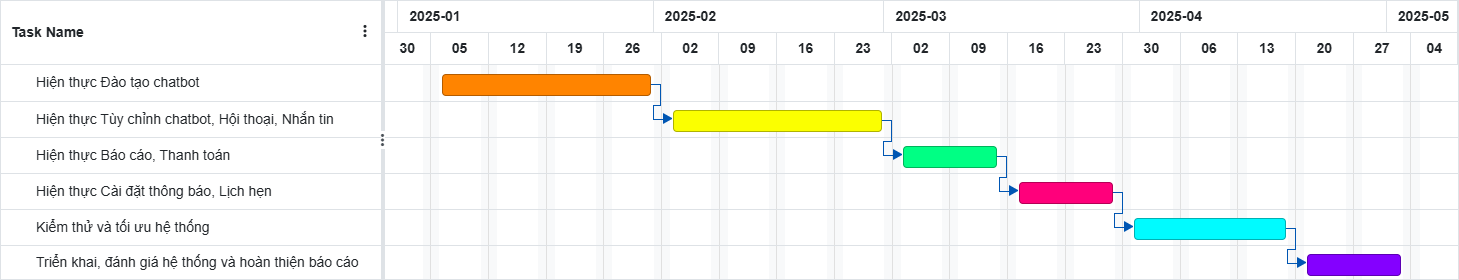
\includegraphics[width=\textwidth]{Images/future_plan.png}
    \vspace{0.5cm}
    \caption{Biểu đồ Gantt kế hoạch triển khai dự án}
    \label{fig:gantt-chart}
\end{figure}

\textbf{1. Nhân sự thực hiện:}
\begin{itemize}
    \item Frontend Engineer: Lê Đình Huy
    \begin{itemize}
        \item Phụ trách phát triển giao diện người dùng
        \item Đảm bảo trải nghiệm người dùng (UX/UI)
    \end{itemize}
    \item Backend Engineer: Phạm Đức Thắng
    \begin{itemize}
        \item Phụ trách phát triển API và xử lý logic nghiệp vụ
        \item Quản lý cơ sở dữ liệu và bảo mật hệ thống
    \end{itemize}
    \item AI Engineer: Nguyễn Đức An
    \begin{itemize}
        \item Phụ trách phát triển và tích hợp các mô hình AI
        \item Tối ưu hóa hiệu suất xử lý ngôn ngữ tự nhiên
    \end{itemize}
\end{itemize}


\textbf{2. Kế hoạch chi tiết theo giai đoạn:} \\

\textbf{Giai đoạn 1: Phát triển module đào tạo chatbot} (6/1-2/2/2025)
\begin{itemize}
    \item Nội dung và phân công:
    \begin{itemize}
        \item Frontend Engineer: Hiện thực giao diện đào tạo chatbot
        \item Backend Engineer: Phát triển API đào tạo chatbot
        \item AI Engineer: Tích hợp và tối ưu mô hình AI cho chatbot
    \end{itemize}
    \item Kết quả mong đợi:
    \begin{itemize}
        \item Hoàn thiện module đào tạo chatbot có khả năng tương tác với AI
        \item Giao diện người dùng thân thiện và dễ sử dụng
    \end{itemize}
\end{itemize}

\textbf{Giai đoạn 2: Xây dựng tính năng tùy chỉnh và tương tác} (3/2-2/3/2025)
\begin{itemize}
    \item Nội dung và phân công:
    \begin{itemize}
        \item Frontend Engineer: Phát triển giao diện tùy chỉnh chatbot và hội thoại
        \item Backend Engineer: Xây dựng API tích hợp với website và Facebook
        \item AI Engineer: Tối ưu hóa khả năng xử lý ngôn ngữ tự nhiên
    \end{itemize}
    \item Kết quả mong đợi:
    \begin{itemize}
        \item Hệ thống chatbot tích hợp đa nền tảng
        \item Khả năng tùy chỉnh linh hoạt theo nhu cầu người dùng
    \end{itemize}
\end{itemize}

\textbf{Giai đoạn 3: Phát triển hệ thống báo cáo và thanh toán} (3-16/3/2025)
\begin{itemize}
    \item Nội dung và phân công:
    \begin{itemize}
        \item Frontend Engineer: Xây dựng giao diện báo cáo và thanh toán
        \item Backend Engineer: Phát triển API thanh toán và tích hợp cổng thanh toán
        \item AI Engineer: Phát triển các thuật toán phân tích dữ liệu cho báo cáo
    \end{itemize}
    \item Kết quả mong đợi:
    \begin{itemize}
        \item Hệ thống báo cáo chi tiết và trực quan
        \item Tích hợp thanh toán an toàn và đa dạng
    \end{itemize}
\end{itemize}

\textbf{Giai đoạn 4: Xây dựng tính năng thông báo và lịch hẹn} (17-30/3/2025)
\begin{itemize}
    \item Nội dung và phân công:
    \begin{itemize}
        \item Frontend Engineer: Phát triển giao diện quản lý thông báo và lịch hẹn
        \item Backend Engineer: Xây dựng API quản lý thông báo và lịch hẹn
        \item AI Engineer: Tích hợp thuật toán gợi ý thời gian hẹn tối ưu
    \end{itemize}
    \item Kết quả mong đợi:
    \begin{itemize}
        \item Hệ thống thông báo thời gian thực
        \item Quản lý lịch hẹn hiệu quả
    \end{itemize}
\end{itemize}

\textbf{Giai đoạn 5: Kiểm thử và tối ưu hóa} (31/3-20/4/2025)
\begin{itemize}
    \item Nội dung và phân công:
    \begin{itemize}
        \item Frontend Engineer: Kiểm thử UI/UX và tối ưu giao diện
        \item Backend Engineer: Kiểm thử API và tối ưu hiệu suất hệ thống
        \item AI Engineer: Tối ưu hóa các mô hình AI và đánh giá độ chính xác
    \end{itemize}
    \item Kết quả mong đợi:
    \begin{itemize}
        \item Độ ổn định và hiệu suất cao của hệ thống
        \item Phát hiện và khắc phục các lỗi tiềm ẩn
    \end{itemize}
\end{itemize}

\textbf{Giai đoạn 6: Triển khai và hoàn thiện} (21/4-4/5/2025)
\begin{itemize}
    \item Nội dung và phân công:
    \begin{itemize}
        \item Frontend Engineer: Triển khai giao diện người dùng
        \item Backend Engineer: Triển khai hệ thống backend lên cloud
        \item AI Engineer: Triển khai các mô hình AI và monitoring
    \end{itemize}
    \item Kết quả mong đợi:
    \begin{itemize}
        \item Hệ thống hoạt động ổn định trên môi trường thực tế
        \item Báo cáo đồ án hoàn chỉnh và chuyên nghiệp
    \end{itemize}
\end{itemize}